% CVPR 2025 Paper Template; see https://github.com/cvpr-org/author-kit

\documentclass[10pt,twocolumn,letterpaper]{article}

%%%%%%%%% PAPER TYPE  - PLEASE UPDATE FOR FINAL VERSION
% \usepackage{cvpr}              % To produce the CAMERA-READY version
\usepackage[]{cvpr}      % To produce the REVIEW version
% \usepackage[pagenumbers]{cvpr} % To force page numbers, e.g. for an arXiv version
\usepackage{algorithm}
\usepackage[noend]{algpseudocode}

% Import additional packages in the preamble file, before hyperref
\input{preamble}

% It is strongly recommended to use hyperref, especially for the review version.
% hyperref with option pagebackref eases the reviewers' job.
% Please disable hyperref *only* if you encounter grave issues, 
% e.g. with the file validation for the camera-ready version.
%
% If you comment hyperref and then uncomment it, you should delete *.aux before re-running LaTeX.
% (Or just hit 'q' on the first LaTeX run, let it finish, and you should be clear).
\definecolor{cvprblue}{rgb}{0.21,0.49,0.74}
\usepackage[pagebackref,breaklinks,colorlinks,allcolors=cvprblue]{hyperref}

%%%%%%%%% PAPER ID  - PLEASE UPDATE
\def\paperID{1} % *** Enter the Paper ID here
\def\confName{CVPR}
\def\confYear{2025}

%%%%%%%%% TITLE - PLEASE UPDATE
\title{TicTacZero: A TicTacToe Engine}

%%%%%%%%% AUTHORS - PLEASE UPDATE
\author{Anish Chandra\\
University of Michigan-Ann Arbor\\
{\tt\small anishcha@umich.edu}
% For a paper whose authors are all at the same institution,
% omit the following lines up until the closing ``}''.
% Additional authors and addresses can be added with ``\and'',
% just like the second author.
% To save space, use either the email address or home page, not both
% \and
% Second Author\\
% Institution2\\
% First line of institution2 address\\
% {\tt\small secondauthor@i2.org}
}

\begin{document}
\maketitle   
\input{sec/1_intro}
\input{sec/2_relatedwork}
\section{Method}

This section consists of all the design decisions for this engine. This engine implements many of the same as the AlphaGo Zero model, however, due to the different nature of TicTacToe, there are some important alterations to the overall paradigm to be discussed. More specifically, there are three main sections: Monte Carlo Tree Search, the Policy and Value Networks, and finally, self-play training.
%--------------------------------------------------------------------------------------------
\subsection{Monte Carlo Tree Search}
Intuitively, most board games can be devolved down to a simple tree, where the edges are actions and the vertices are the resulting board states. A brute force solution to an engine for these board games is to search for all winning states any arbitrary move can lead to, and pick the move that maximizes the total number of winning states. However, this search operation poorly scales with any increase in action possibilities. Hence when playing complicated games, some optimization is necessary. 

The primary optimization that MCTS makes is done by introducing a heuristic. More specifically, it performs a search by running simulations of games by selecting moves using the metric known as the Upper Confidence Bound or the $UCB$ score, formulated in \cref{sec:ucb_score}.

A simulation consists of moves starting from the current state and proceeding by greedily selecting moves using the score until it reaches an undiscovered state of the game. Once it reaches this undiscovered state, it will expand the node (by connecting all possible moves as children), and determine the value of the node. This value is finally then backpropagated through the search path by offsetting each of the nodes' current value by this new value. Note that this is a very rough description of the algorithm, the more formalized pseudocode can be referenced in \cref{sec:mcts_code}.


% Store the equation in the appendix.
% \begin{equation}
%   UCB_1(v_{parent}, v_{child}) = \begin{cases}
%     p_{child}(\frac{\sqrt{n_{parent}}}{n_{child} + 1}) -  \quad &\text{if} \, n_{child} > 0 \\
%     -x \quad &\text{if} \, n_{child} \leq 0 \\
%   \end{cases}
% \end{equation}

%--------------------------------------------------------------------------------------------

\subsection{Policy and Value}
Recall that the $UCB$ score depends on some prior probabilities and values. When a state is undetermined (i.e. neither player has won), its value and priors are determined by 2 neural networks: the Policy and Value. Although these terms are prominently used in RL, in this situation, it can be simplified to be the answers of two questions. The policy network answers how likely each action is to lead to a winning state, and the value network answers how \textit{winnable} a state of the game is. This information is then fed into MCTS in the form of the $UCB$ score to determine how \emph{helpful} a move may be to investigate.

Since TicTacToe is a simple game, the model reflects the same. The model is a standard Feedforward Neural Network with 2 hidden layers, each with 16 neurons and ReLU applied. Finally, there are two output heads: a policy head (9 neurons) and a value head (1 neuron), of which, have applied log-softmax and the sigmoid activation functions (augmented to go from $-1\to1$), respectively.

To determine the loss it can be observed that the policy is effectively a vector of classification probabilities. As such this paper uses a variant of Categorical Cross Entropy loss, defined as the following equation:
\begin{equation}
  L_{cross-entropy} = -\sum_{i}y_i\log(\hat y_i)
\end{equation}
Likewise, the loss for the value function is the Mean Squared Error (MSE) loss, as it's effectively comparing two scalars.

\subsection{Self-Play Training}
One of the key features of this engine, is that it requires no human generated examples and only relies on playing itself, thereby allowing it to develop its own novel strategies. The algorithm works by repeatedly performing the following:
\begin{enumerate}
  \item Let the model play itself in \emph{episodes}
  \item Store 3-entry tuples with the state of the game, true action probability output by MCTS, and  value of who won
  \item Train the model on the examples
\end{enumerate}
Note that the MCTS determines the true action probabilities by the number of visits for each child node divided by the number of visits of its parent.

However, there is a case for human generated data as it creates a diversity in the training set of game states. Without this, as soon as the model is shown a game state that it hasn't seen, it will start to make poorly judged moves. In order to suggest the model to diversify its strategies, and potentially lose more often during training, this paper introduces the exploration factor. This factor is used to convert the number of visits a node has, into a more uniform probability distribution, $P$. More mathematically:
\begin{align}
  P(i) &= \frac{x_i^{1/T}}{\sum_{j}x_j^{1/T}} \quad \text{where,}\\
  T &= \text{ exploration factor} \\
  x_i &= i^{th}\text{ action's visit count}
\end{align}

Then the model samples from this distribution to output its \emph{likely best} move. Thus, the model is forced to see more diverse boards and learn newer strategies.
\section{Experiment}
This section describes the more specific implementation process that this engine required. This process is divided into two sections: hyperparameter tuning and the performance of the model against the brute force approach, minimax.

% \subsection{Model Development}
% AlphaGo originally used independent CNNs as the policy and value networks, and initially, this paper did as well. However, there are two primary issues that must be considered for this paper. The first is that both policy and value networks are dealing with the same information, and only differentiated in its output. Hence, the combination of the networks would (and did) perform significantly better than split apart as it becomes effectively the same as transfer learning with replacement of the last layer. The second issue is that TicTacToe is not necessarily a big board game, the $3\times 3$ board doesn't require a lot of spatial comprehension, and thus, the faster and equally proficient FNN is more reasonable.

\subsection{Hyperparameter Tuning}
The hyperparameters for the overall engine was developed to balance the training duration and exploration. In other words, training shouldn't take hours, however, the engine should be given the chance to see varying boards. To do so, the training process involves 30 sets, each consisting of 100 episodes (games), where the model is trained for 50 epochs per set. This sets training time to $\sim$10 minutes, while exposing to up to $\sim$22500 boards (not unique).

The policy and value networks are trained using the Adam optimizer, set with a learning rate of $5\cdot 10^{-4}$ to allow a slow and smooth convergence. Finally, the MCTS exploration factor was set to 4, encouraging a more diverse set of training examples. The effects of these choices can be viewed in the loss plot, in \cref{sec:loss_plot}. 
% Notably, the model from training set 3, which exhibited the least overfitting, was selected for training.

% The main hyperparameters are dealing with training duration. This algorithm needs to promote a lot of game state training examples, it needs to be able to properly investigate future moves, as well as repeat the training process in a reasonable amount of time. With these requirements, this paper found that the optimal durations are: 30 training sets, each running 100 episodes (games), and training the model over these episodes over 50 epochs. Finally, the policy and value FNN model uses the Adam optimizer with learning rate of $5\cdot 10^{-4}$, and run the MCTS algorithm with a exploration factor of 4. With this tuning, the loss graph in \cref{sec:loss_plot} was achieved. From the graph, the model developed from training set 3 was used for testing, as it faced the least over-fitting.

\subsection{Competing with Minimax}
TicTacToe was primarily chosen due to its nature to be easily solved with a brute force algorithm, minimax. While out of scope, minimax is an algorithm that tries to maximize the reward on its own turn, while minimizing the reward on opponent's turns. Since there are only $3^9 = 19683$ boards (even less due to terminal states), it is reasonable to run this brute force approach. For more details on how the algorithm functions, reference the pseudo code in \cref{sec:minimax_code}, however, for this paper, assume it as the \emph{perfect} algorithm to benchmark TicTacZero.

When pitted against TicTacZero, the minimax algorithm could only surely win $30\%$ of the time, giving TicTacZero a $70\%$ win-tie rate over 100 games.
\section{Conclusion}
In conclusion, TicTacZero is a model that was able to learn an optimal strategy, such that it was able to compete with a mathematically correct algorithm. This means that even without human training data, models are able to build themselves up, without the requirement of pre-labeled training data. This paper can safely conclude that the training paradigm provided and built by AlphaGo Zero is applicable across a variety of games/environments. A primary suggestion for future work would be determining a way to teach the model the difference between valid and invalid moves (i.e. determine a way to not require the filtration of invalid moves).
{
    \small
    \bibliographystyle{ieeenat_fullname}
    \bibliography{main}
}
\appendix
\clearpage
\setcounter{page}{1}
\maketitlesupplementary



\section{Computing the Upper Confidence Bound Score of a Game State}
\label{sec:ucb_score}
% Store the equation in the appendix.
The $UCB$ score is an intuitive equation, it promotes exploration and exploitation. It's derived based on following four relations:
\begin{enumerate}
  \item Higher prior $p$ (given by the policy) should \emph{raise} the score
  \item Higher number of times the node's parent has been visited $n_{parent}$, should \emph{raise} the score.
  \item Higher number of times this node has been visited, $n$, should \emph{lower} the score
  \item Higher ratio of value per visits, $V$, of this node, should \emph{lower} the score
\end{enumerate}
\begin{align}
  UCB &= V + P \\
  V &= \begin{cases}
    -\sum_{v\in children} \frac{v}{n} &\quad \text{if} \, n > 0 \\
    0 &\quad \text{otherwise}
  \end{cases} \\
  P &= \frac{p\sqrt{n_{parent}}}{n + 1}
\end{align}

\section{Pseudocode for the Monte Carlo Tree Search}
\label{sec:mcts_code}

\begin{algorithm}[h]
  \caption{Monte Carlo Tree Search (MCTS)}
  \label{alg:mcts}
  \begin{algorithmic}[1]
  \Function{run\_simulations}{$n_{sims}$}
  \State Initialize root node with the current game state.
  \For{$n_{sims}$}
      \State current\_node $\gets$ root
      \State Intialize search\_path to empty list
      \While{current\_node isn't expanded}
          \State Select the next node based on $UCB$
          \State Add the selected node to the search\_path
      \EndWhile
      \If{the game ends at the current node}
          \State value $\gets 1$ if model wins, $-1$ otherwise
      \Else
          \State Expand the current node and predict value
      \EndIf
      \State Add the value to nodes along the search path.
  \EndFor
  \State Compute probabilities for each action based on visit counts.
  \State Select the action with the highest visit count as the best move.
  \State \Return the best action and its probabilities.
  \EndFunction
  \end{algorithmic}
  \end{algorithm}

\section{Loss Plot}
\label{sec:loss_plot}
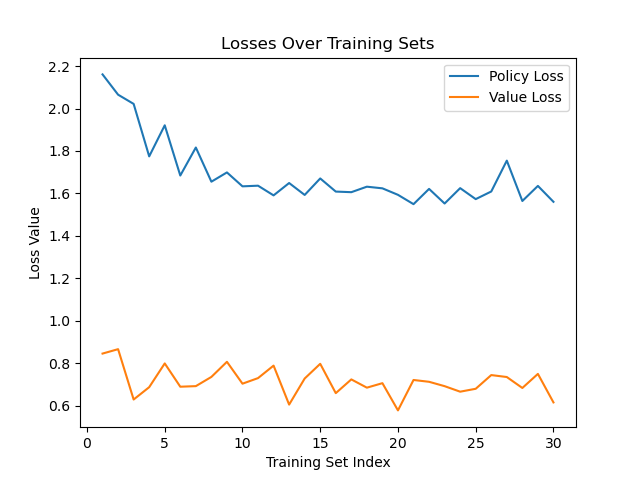
\includegraphics[width=\linewidth]{plots/correct_loss.png}

\section{Pseudocode for the Minimax Algorithm}
\label{sec:minimax_code}
\begin{algorithm}[h]
  \caption{Minimax Algorithm for Tic-Tac-Toe}
  \begin{algorithmic}[1]
  
  \Function{Score}{board, $depth$}
      \If{PlayerWins(board)}
          \State \Return $10 - depth$
      \ElsIf{OpponentWins(board)}
          \State\Return $-10 + depth$
      \Else
          \State\Return 0
      \EndIf
  \EndFunction

  \Function{Minimax}{board, depth, isPlayer}
      \If{GameOver(board)}
          \State\Return{Score(board, depth)}
      \EndIf
      
      \State{moves} $\gets$ GetValidMoves(board)
      
      % \For{each move in moves}
      %     \State{newBoard} $\gets$ MakeMove(board, move)
      %     \State{score} $\gets$ Minimax(newBoard, depth + 1, $\neg$isPlayer)
          
      %     \If{isMaximizer}
      %         \If{score > bestScore}
      %             \State{bestScore} $\gets$ score
      %             \State{bestMove} $\gets$ move
      %         \EndIf
      %     \Else
      %         \If{score < bestScore}
      %             \State{bestScore} $\gets$ score
      %             \State{bestMove} $\gets$ move
      %         \EndIf
      %     \EndIf
      % \EndFor
      \State Initialize scores as a list
      \For{each move in moves}
        \State Initialize newBoard with move
        \State scores $\gets$ Minimax(newBoard, depth+1 $\neg$ isPlayer)
      \EndFor
      \If{isPlayer}
        \State \Return move and score that maximizes score
      \Else
        \State \Return move and score that minimizes score
      \EndIf
  \EndFunction
  
  \end{algorithmic}
  \end{algorithm}

% \section{Policy and Value Network Diagrams}
% 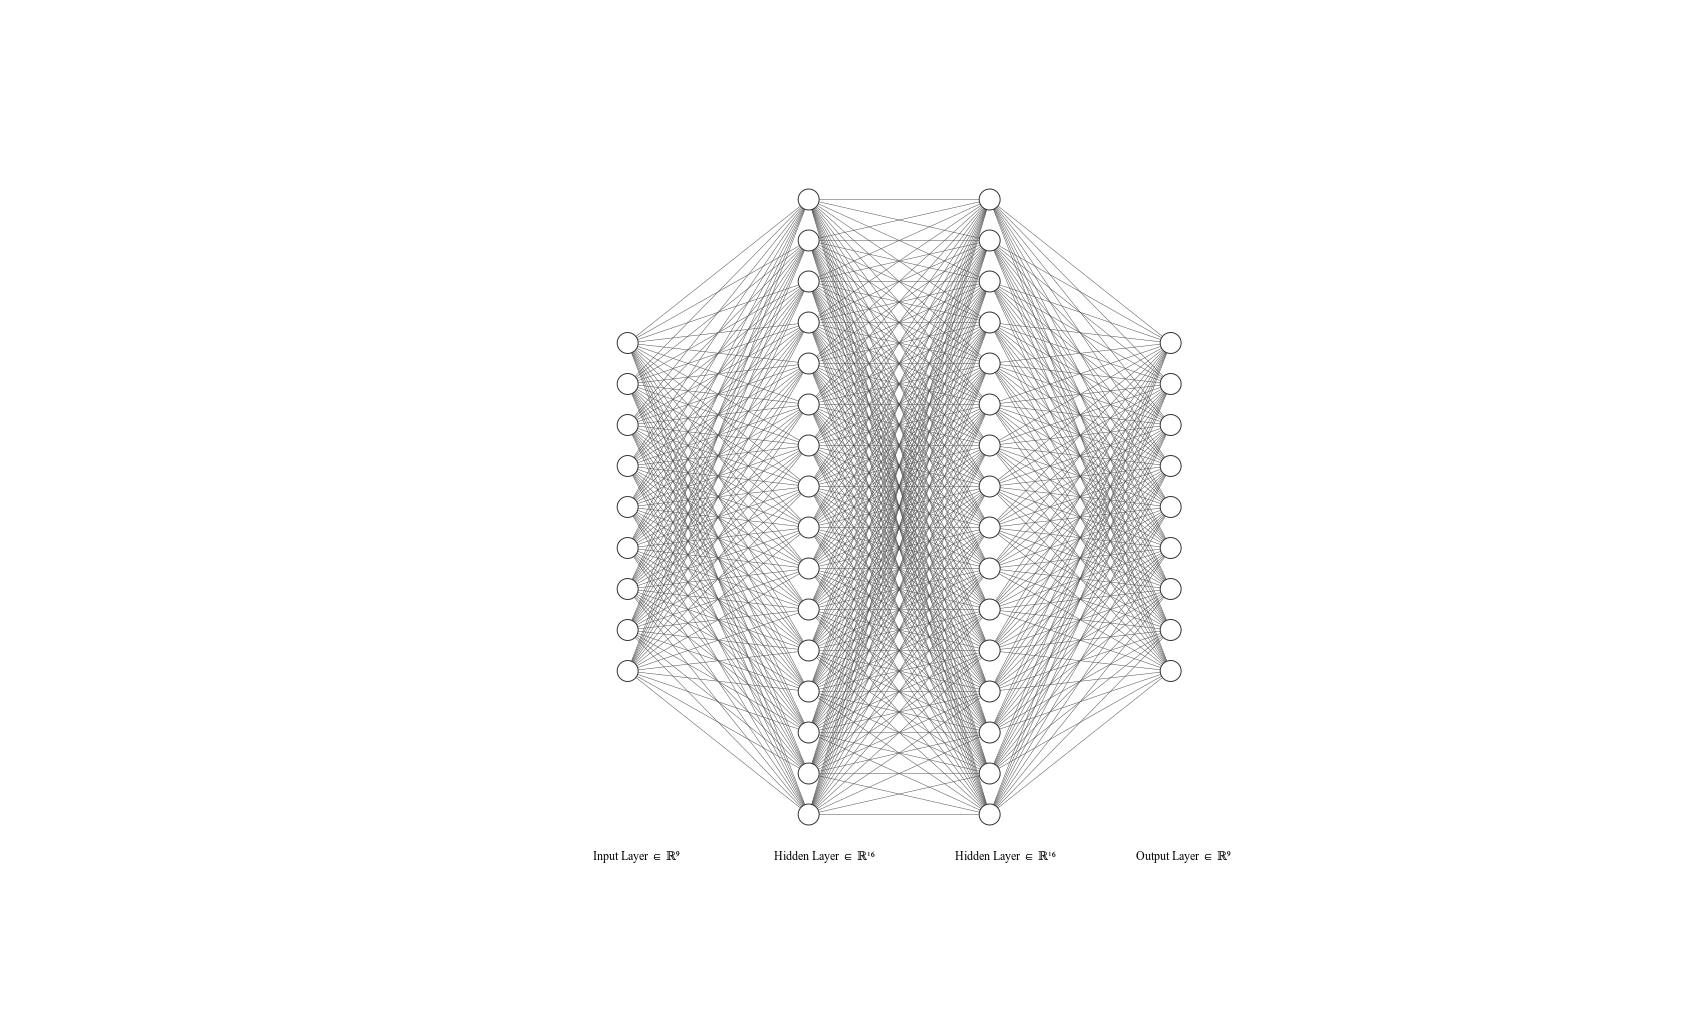
\includegraphics[width=\linewidth]{plots/policy.png}
% 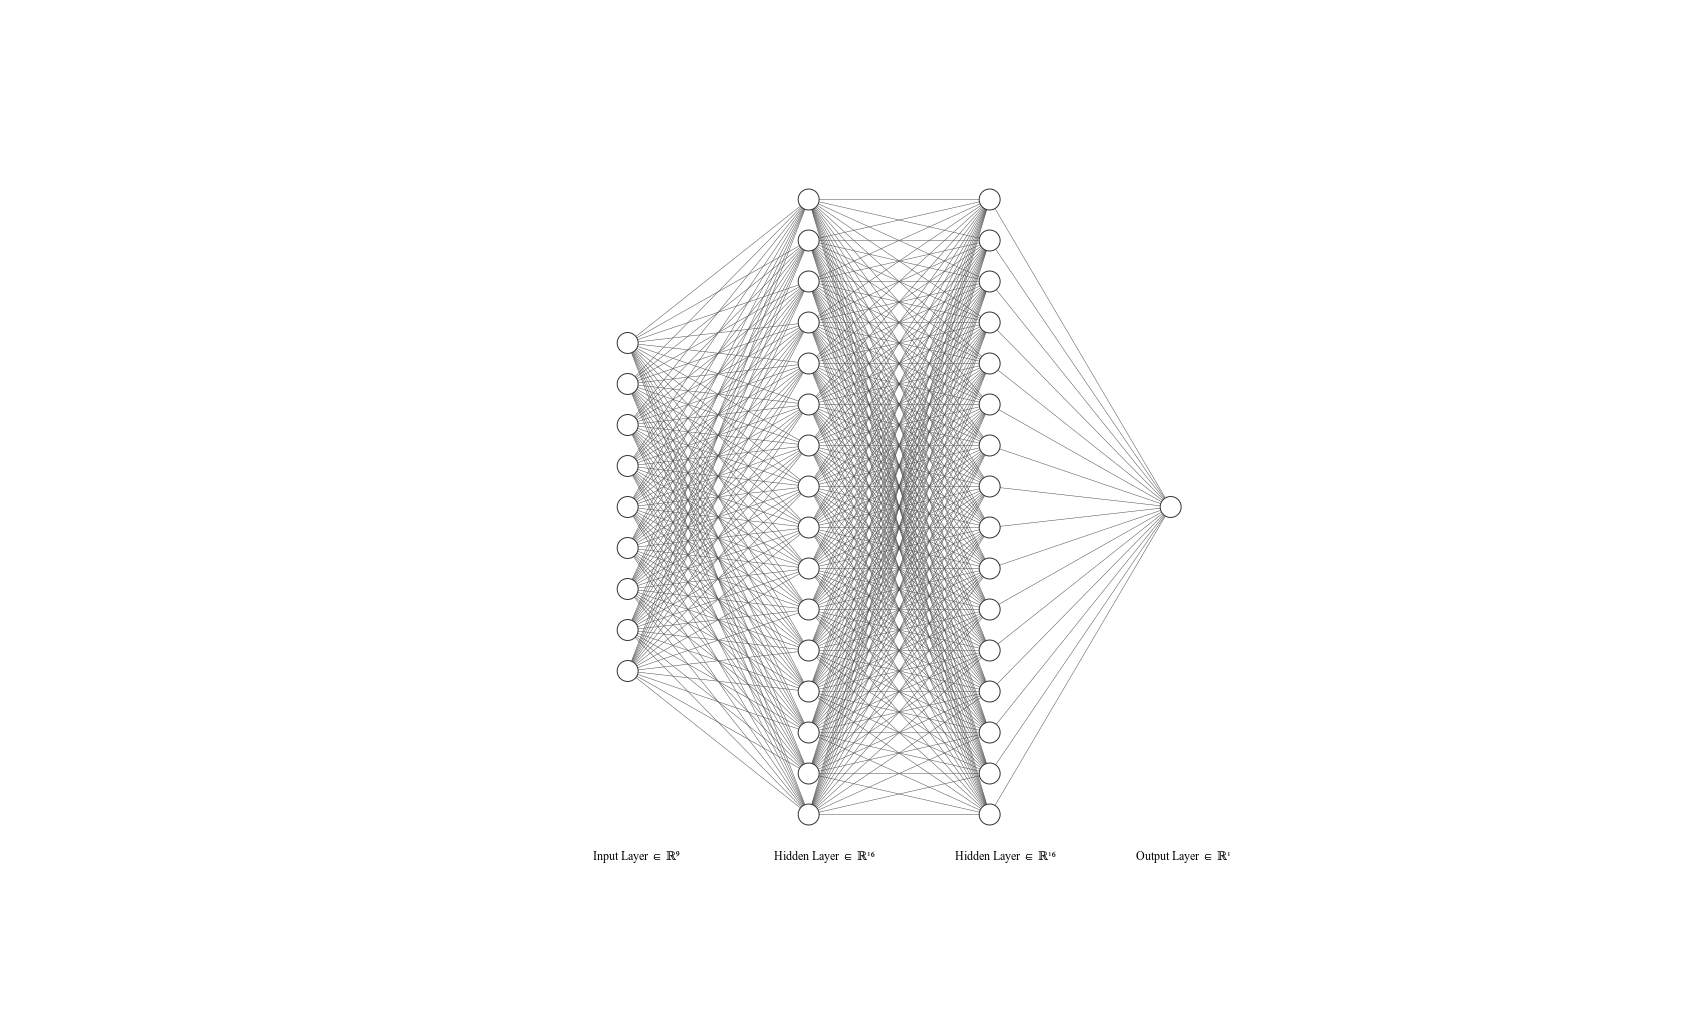
\includegraphics[width=\linewidth]{plots/value.png}

% WARNING: do not forget to delete the supplementary pages from your submission 
% \input{sec/X_suppl}

\end{document}
